
\chapter{Introduction}

\chapterquote{%
It must be admitted that the use of geometric intuition has no logical
necessity in mathematics, and is often left out of the formal presentation
of results.  If one had to construct a mathematical brain, one would
probably use resources more efficiently than creating a visual system.  But
the system is there already, it is used to great advantage by human
mathematicians, and it gives a special flavor to human mathematics.}{%
Ruelle~\cite{Rue}}



\noindent
Higher-dimensional category theory is the study of a zoo of exotic
structures: operads, $n$-categories, multicategories, monoidal categories,
braided monoidal categories, and more.  It is intertwined with the study of
structures such as homotopy algebras ($A_\infty$-categories,
$L_\infty$-algebras, $\Gamma$-spaces, \ldots), $n$-stacks, and $n$-vector
spaces, and draws it inspiration from areas as diverse as topology, quantum
algebra, mathematical physics, logic, and theoretical computer science.

No surprise, then, that the subject has developed chaotically.  The rush
towards formalizing certain commonly-imagined concepts has resulted in an
extraordinary mass of ideas, employing diverse techniques from most of the
subject areas mentioned.  What is needed is a transparent, natural, and
practical language in which to express these ideas.

The main aim of this book is to present one.  It is the language of
generalized operads.  It is introduced carefully, then used to give simple
descriptions of a variety of higher categorical structures.

I hope that by the end, the reader will be convinced that generalized
operads provide as appropriate a language for higher-dimensional category
theory as vector spaces do for linear algebra, or sheaves for algebraic
geometry.  Indeed, the reader may also come to share the feeling that
generalized operads are as applicable and pervasive in mathematics at large
as are $n$-categories, the usual focus of higher-dimensional category
theorists.

Here are some of the structures that we will study, presented informally.

Let $n\in\nat$.  An \demph{$n$-category}%
%
\index{n-category@$n$-category!definitions of!informal}
%
consists of \demph{$0$-cells}%
%
\index{cell!n-category@of $n$-category}
%
(objects) $a, b, \ldots$, \demph{$1$-cells}
(arrows) $f, g, \ldots$, \demph{$2$-cells} (arrows between arrows) $\alpha,
\beta, \ldots$, \demph{$3$-cells} (arrows between arrows between arrows)
$\Gamma, \Delta, \ldots$, and so on, all the way up to \demph{$n$-cells},
together with various composition operations.  The cells are usually drawn
like this:
\[
\gzero{a},
\ \ 
\gfst{a}\gone{f}\glst{b},
\ \ 
\gfst{a}\gtwomult{f}{g}{\alpha}\glst{b},
\ \ 
\gfst{a}\gthreecellmult{f}{g}{\alpha}{\beta}{\Gamma}\glst{b},
\ \ 
\ldots.
\]
Typical example: for any topological space $X$ there is an $n$-category whose
$k$-cells are maps from the closed $k$-dimensional ball into $X$.  A
$0$-category%
%
\index{zero-category@0-category}
%
is just a set, and a $1$-category%
%
\index{one-category@1-category}
%
just an ordinary category.

A \demph{multicategory}%
%
\index{multicategory!informal definition of}
%
consists of objects $a, b, \ldots$, arrows $\theta,
\phi, \ldots$, a composition operation, and identities, just like an
ordinary category, the difference being that the domain of an arrow is not
just a single object but a finite sequence of them.  An arrow is therefore
drawn as
\[
\begin{centredpic}
\begin{picture}(8,4)(-2,-2)
\cell{0}{0}{l}{\tusual{\theta}}
\cell{0}{0}{r}{\tinputsslft{a_1}{a_2}{a_k}}
\cell{4}{0}{l}{\toutputrgt{a}}
\end{picture}
\end{centredpic}
\]
(where $k\in\nat$), and composition turns a tree of arrows into a single
arrow.  Vector spaces and linear maps form a category; vector spaces and
multilinear maps form a multicategory.

An \demph{operad}%
%
\index{operad!informal definition of}
%
is a multicategory with only one object.
Explicitly, an operad consists of a set $P(k)$ for each $k\in\nat$, whose
elements are thought of as `$k$-ary operations' and drawn as
\[
\begin{centredpic}
\begin{picture}(8,4)(-2,-2)
\cell{0}{0}{l}{\tusual{\theta}}
\cell{0}{0}{r}{\tinputsslft{}{}{}}
\cell{4}{0}{l}{\toutputrgt{}}
\end{picture}
\end{centredpic}
\]
with $k$ input wires on the left, together with a rule for composing the
operations and an identity operation.  Example: for any vector space $V$
there is an operad whose $k$-ary operations are the linear maps $V^{\otimes
k} \go V$.

Operads describe operations%
%
\index{operation}%
%
\index{arrow}
%
that take a finite sequence of things as input
and produce a single thing as output.  A finite sequence is a 1-dimensional
entity, so operads can be used, for example, to describe the operation of
composing a (1-dimensional) string of arrows in a (1-)category.  But if we
are interested in higher-dimensional structures such as $n$-categories
then we need a more general notion of operad, one where the inputs of an
operation can form a higher-dimensional shape---a grid, perhaps, or a tree,
or a so-called pasting diagram.  For each choice of `input type'%
%
\index{input type}
%
$T$, there
is a class of \demph{$T$-operads}.%
%
\index{generalized operad!informal definition of}
%
 A $T$-operad consists of a family of
operations whose inputs are of the specified type, together with a rule for
composition; for instance, if the input type $T$ is `finite sequences' then
a $T$-operad is an ordinary operad.  Fig.~\ref{fig:T-examples} shows
typical operations $\theta$ in a $T$-operad, for four different choices of
$T$.
%
\begin{figure}\centering
\[
\begin{array}{ccc}
\begin{array}{c}
\setlength{\unitlength}{1em}
\begin{picture}(8,4)(-2,-2)
\cell{0}{0}{l}{\tusual{\theta}}
\cell{0}{1.5}{r}{\tinputlft{}}
\cell{0}{0.75}{r}{\tinputlft{}}
\cell{0}{0}{r}{\tinputlft{}}
\cell{0}{-0.75}{r}{\tinputlft{}}
\cell{0}{-1.5}{r}{\tinputlft{}}
\cell{4}{0}{l}{\toutputrgt{}}
\end{picture}
\end{array}
&&
\begin{array}{c}
\includegraphics{domtreeop.eps}
\end{array}
\goby{\textstyle\theta}
\begin{array}{c}
\includegraphics{codtreeop.eps}
\end{array}
\\
\\
\begin{array}{c}
\setlength{\unitlength}{1em}
\begin{picture}(5.4,3.6)
\put(0,0){\line(1,0){5.4}}
\put(0,1.8){\line(1,0){5.4}}
\put(0,3.6){\line(1,0){5.4}}
\put(0,0){\line(0,1){3.6}}
\put(1.8,0){\line(0,1){3.6}}
\put(3.6,0){\line(0,1){3.6}}
\put(5.4,0){\line(0,1){3.6}}
\cell{0.9}{0.9}{c}{\Downarrow}
\cell{2.7}{0.9}{c}{\Downarrow}
\cell{4.5}{0.9}{c}{\Downarrow}
\cell{0.9}{2.7}{c}{\Downarrow}
\cell{2.7}{2.7}{c}{\Downarrow}
\cell{4.5}{2.7}{c}{\Downarrow}
\end{picture}
\end{array}
\goby{\textstyle\theta}
\begin{array}{c}
\setlength{\unitlength}{1em}
\begin{picture}(1.8,1.8)
\put(0,0){\line(1,0){1.8}}
\put(0,1.8){\line(1,0){1.8}}
\put(0,0){\line(0,1){1.8}}
\put(1.8,0){\line(0,1){1.8}}
\cell{0.9}{0.9}{c}{\Downarrow}
\end{picture}
\end{array}
&&
\gfstsu\gthreemultsu\gzersu\gfourmultsu\glstsu
\goby{\textstyle\theta}
\gfstsu\gtwomultsu\glstsu
\end{array}
\]
\caption{Operations $\theta$ in four different types of generalized operad}
\label{fig:T-examples}
\end{figure}
% 
Similarly, there are \demph{$T$-multicategories},%
%
\index{generalized multicategory!informal definition of}
%
where the shapes at the
domain and codomain of arrows are labelled with the names of objects.
These are the `generalized operads' and `generalized multicategories'
at the heart of this book.

The uniting feature of all these structures is that they are purely
algebraic in definition, yet near-impossible to understand without drawing
or visualizing pictures.  They are inherently geometrical.  

A notorious problem in this subject is the multiplicity of definitions of
$n$-category.%
%
\index{n-category@$n$-category!definitions of!comparison}
%
 Something like a dozen different definitions have been
proposed, and there are still very few precise results stating equivalence
between any of them.  This is not quite the scandal it may seem: it is hard to
say what `equivalence'%
%
\index{equivalence!definitions of n-category@of definitions of $n$-category}
%
should even mean.  Suppose that Professors X and Y
each propose a definition of $n$-category.  To compare their definitions,
you find a way of taking one of X's $n$-categories and deriving from it
one of Y's $n$-categories, and vice-versa, then you try to show that
doing one process then the other gets you back to where you started.  It
is, however, highly unrealistic to expect that you will get back to
\emph{exactly} where you started.  For most types of mathematical
structure, getting back to somewhere isomorphic to your starting point
would be a reasonable expectation.  But for $n$-categories, as we shall
see, this is still unrealistic: the canonical notion of equivalence%
%
\index{equivalence!n-categories@of $n$-categories}
%
of
$n$-categories is much weaker than isomorphism.  Finding a precise
definition of equivalence for a given definition of $n$-category can be
difficult.  Indeed, many of the proposed definitions of $n$-category did
not come with accompanying proposed definitions of equivalence, and this
gap must be almost certainly be filled before any comparison results can be
proved.


Is this all `just language'?  There would be no shame if it were: language
can have the most profound effect.  New language can make new concepts
thinkable, and make old, apparently obscure, concepts suddenly seem natural
and obvious.  But there is no clear line between mathematical language and
`real' mathematics.  For example, we will see that a 3-category%
%
\index{three-category@3-category!degenerate}
%
with only
one 0-cell and one 1-cell is precisely a braided monoidal category,%
%
\index{monoidal category!braided!degenerate}
%
and
that the free braided monoidal category on one object is the sequence
$(B_n)_{n\in\nat}$ of braid%
%
\index{braid}
%
groups.  So if $n$-categories are just
language, not `real' mathematical objects, then the same is true of the
braid groups, which describe configurations of knotted string.  The
distinction begins to look meaningless.

Here is a summary of the contents.


\subsection*{Motivation for topologists}

Topology and higher-dimensional category theory are intimately related.
The diagrams that one cannot help drawing when thinking about higher
categorical structures can very often be taken literally as pieces of
topology.  We start with an informal discussion of the connections between
the two subjects.  This includes various topological examples of
$n$-categories, and an account of how the world of $n$-categories is a
mirror of the world of homotopy groups of spheres.


\subsection*{Part~\ref{part:background}: Background}

We will build on various `classical' notions.  Those traditionally
considered the domain of category theorists are in
Chapter~\ref{ch:classical}: ordinary categories, bicategories, strict
$n$-categories, and enrichment.  Classical operads and multicategories have
Chapter~\ref{ch:om} to themselves.  They should be viewed as categorical
structures too, although, anomalously, operads are best known to homotopy
theorists and multicategories to categorical logicians.

The familiar concept of monoidal (tensor) category can be formulated in a
remarkable number of different ways.  We look at several in
Chapter~\ref{ch:monoidal}, and prove them equivalent.  Monoidal categories
can be identified with one-object 2-categories, so this is a microcosm of
the comparison of different definitions of $n$-category.



\subsection*{Part~\ref{part:operads}: Operads} 

This introduces the central idea of the text: that
of generalized (`higher') operad and multicategory.  The definitions---of
generalized operad and multicategory, and of algebra for a generalized operad
or multicategory---are stated and explained in
Chapter~\ref{ch:gom-basics}, and some further theory is developed in
Chapter~\ref{ch:gom-further}.  

There is a truly surprising theory of enrichment%
%
\index{enrichment!generalized multicategory@of generalized multicategory}%
%
\index{generalized multicategory!enriched}
%
for generalized
multicategories---it is not at all the routine extension of traditional
enriched category theory that one might expect.  This was to have formed
Part~IV of the book, but for reasons of space it was (reluctantly) dropped.  A
summary of the theory, with pointers to the original papers, is
in Section~\ref{sec:enr-mtis}.  

The rest of Part~\ref{part:operads} is made up of examples and
applications.  Chapter~\ref{ch:fcm} is devoted to so-called
\fc-multicategories,%
%
\index{fc-multicategory@$\fc$-multicategory}
%
which are generalized multicategories for a certain choice of input shape.
They turn out to provide a clean setting for some familiar categorical
constructions that have previously been encumbered by technical
restrictions.  In Chapter~\ref{ch:opetopic} we look at opetopic sets,
structures analogous to simplicial sets and used in the definitions of
$n$-category proposed by Baez, Dolan, and others.  Again, the language of
higher operads provides a very clean approach; we also find ourselves drawn
inexorably into higher-dimensional topology.


\subsection*{Part~\ref{part:n-categories}: $n$-Categories}

Using the language of generalized operads, some of the proposed definitions
of $n$-category are very simple to state.  We start by concentrating on one
in particular, in which an $n$-category is defined as an algebra for a
certain globular operad.  A globular operad%
%
\index{globular operad!informal definition of}
%
is a $T$-operad for a certain
choice of input type $T$; the associated diagrams are complexes of disks,
as in the last arrow $\theta$ of Fig.~\ref{fig:T-examples}.
Chapter~\ref{ch:globular} explains what globular operads are in pictorial
terms.  In Chapter~\ref{ch:a-defn} we choose a particular globular operad,
define an $n$-category as an algebra for it, and explore the implications
in some depth.  

The many proposed definitions of $n$-category are not as dissimilar as they
might at first appear.  We go through most of them in
Chapter~\ref{ch:other-defns}, drawing together the common threads.



\subsection*{Appendices}

This book is mostly about description: we develop language in which
structures can be described simply and naturally, accurately reflecting
their geometric reality.  In other words, we mostly avoid the convolutions
and combinatorial complexity often associated with higher-dimensional
category theory.  Where things run less smoothly, and in other situations
where a lengthy digression threatens to disrupt the flow of the main text,
the offending material is confined to an appendix.  As long as a few
plausible results are taken on trust, the entire main text can be read and
understood without looking at any of the appendices.




\paragraph*{}

A few words on terminology are needed.  There is a distinction between
`weak' and `strict' $n$-categories,%
%
\index{n-category@$n$-category!weak vs. strict@weak \vs.\ strict}
%
as will soon be explained.  For many
years only the strict ones were considered, and they were known simply as
`$n$-categories'.  More recently it came to be appreciated that weak
$n$-categories are much more abundant in nature, and many authors now use
`$n$-category' to mean the weak version.  I would happily join in, but for
the following obstacle: in most parts of this book that concern
$n$-categories, both the weak and the strict versions are involved and
discussed in close proximity.  It therefore seemed preferable to be
absolutely clear and say either `weak $n$-category' or `strict
$n$-category' on every occasion.  The only exceptions are in this
Introduction and the Motivation for Topologists, where the modern
convention is used.

The word `operad'%
%
\index{operad!usage of word}
%
will be used in various senses.  The most primitive kind
of operad is an operad of sets without symmetric group action, and this is
our starting point (Chapter~\ref{ch:om}).  We hardly ever consider operads
equipped with symmetric group actions, and when we do we call them
`symmetric operads'; see p.~\pageref{p:sym-warning} for a more
comprehensive warning.

Any finite sequence $x_1, \ldots, x_n$ of elements of a monoid has a
product $x_1 \cdots x_n$.  When $n=0$, this is the the unit element.
Similarly, an identity arrow in a category can be regarded as the composite
of a zero-length string of arrows placed end to end.  I have taken the view
throughout that there is nothing special about units or identities; they
are merely nullary%
%
\index{nullary!composite}
%
products or composites.  Related to this is a small but
important convention: the natural%
%
\index{natural number}
%
numbers, $\nat$,%
% 
\glo{nat}
%
start at zero.

